\section{Android}

\subsection{Architecture}
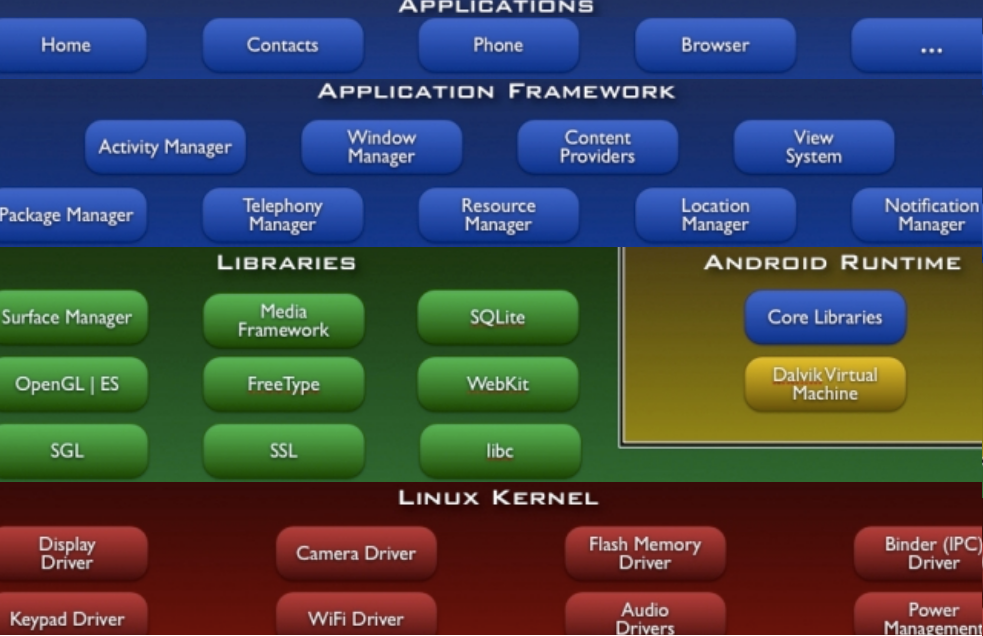
\includegraphics[width=0.15\textwidth]{android/architecture.png}
\textbf{Linux Kernel:} hardware abstraction layer (HAL), device drivers, memory
/ process management, networking

\textbf{Libraries:} C/C++ libraries. Interface through Java. Surface Manager.
2D and 3D Graphics. Media codecs, SQLite, Browser engine

\textbf{Android Runtime:}
Android runtime (ART) and its predecessor Dalvik are the managed runtime used
by apps and some system services.
Executes Dalvik Code (translated from Java bytecode).
Supports Ahead-of-time (AOT) compilation, garbage collections, profiling and
debugging.
Optimized for systems that are constrained in terms of memory and processor
speed.

\textbf{Application Framework:}
API interface, Activity manager (Manages the application life cycle).

\textbf{Applications:}
Built-in and user applications. Can replace built-in applications.

\subsection{Security}
\textbf{Key features}

\textbf{Robust security through a kernel derived from Linux 3.10.x.}
Three-class file system permissions (Prevents user A from reading user B’s
files unless A has group or world privileges). Process isolation (Prevents user
A from exhausting user B’s memory, CPU resources, devices). Extensible
mechanism for secure inter-process communication.

\textbf{Mandatory application sandbox for all applications.}
each app has its own User-ID (UID) and runs as a dedicated process. Rooting the
device and running apps as root breaks security from this sandbox as root has
full access to all application data.

\textbf{Secure inter-process communication}
The Android manifest tells the system which top-level components (activities,
services, etc.) may receive which intents. Services can provide interfaces
directly accessible using binder. Content providers expose data over process
boundaries.


\textbf{Application signing}
Package manager and Google Play verify signatures with public key but do not
verify the Certificate Authority.

\textbf{Application-defined and user-granted permissions}
Sensitive APIs can only be accessed with app-defined and user-granted
permissions. Access without permission yields a security exception.

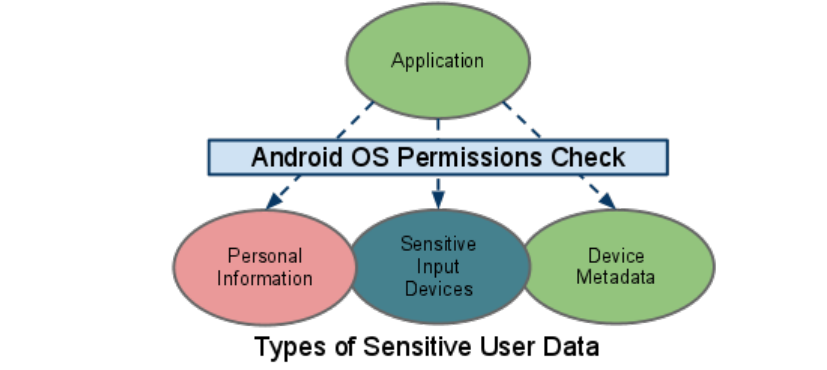
\includegraphics[width=0.15\textwidth]{android/permission_types.png}

important permissions:
\begin{lstlisting}
$READ_EXTERNAL_STORAGE, WRITE_EXTERNAL_STORAGE, INTERNET, CALL_PHONE, WAKE_LOCK,
READ_SMS, RECEIVE_SMS, READ_CONTACTS, ACCESS_FINE_LOCATION, BROADCAST_STICKY$
\end{lstlisting}

\subsubsection{Bouncer}
Google tests apps for malicious behavior through a service called Bouncer (it
tests the app in their cloud infrastructure). Google play remains as of today a
major channel of malware distribution. Majority of infections is through free
illegitimate copies of paid content \textbf{(„re-packaging“)}.

\subsubsection{Exploitability and attack vectors}
\textbf{Worm:} The main objective of this stand-alone type of malware is to endlessly
reproduce itself and spread to other devices

\textbf{Trojan}: a Trojan horse always requires user interaction to be
activated. A Trojan is a kind of virus that is usually inserted into attractive
and seemingly non-malicious executable files or applications that are are
downloaded to the device and executed by the user.

\textbf{Spyware}: This type of malware poses a threat to mobile devices by
collecting, using, and spreading the user's personal or sensitive information
without consent or knowledge

\textbf{Ghost Push}: This is type of malware which infects the Android OS by
automatically gaining root access, downloading malicious software, converting
it to the system app and then losing root access which makes it virtually
impossible to remove the infection by factory reset unless the firmware is
reflashed.

\subsubsection{Native Executable Control}
All current exploit-based attacks depend on the ability to execute native code
outside the Android run-time VM.

\subsubsection{Propagation Scenarios}
Direct self-spreading mechanisms over primary communication networks known from
desktop environments are unlikely. More likely spreading mechanisms involve
Google Play and third party app markets, Websites, Infection via personal
computers, Device-to-device infection, Infection via rogue networks.

\subsubsection{Threat Scenarios}
Information leakage, Online banking fraud, Classical threats such as espionage,
eavesdropping, blackmailing, botnet formation, Botnet Scenarios.

\subsection{Components}
App is built of Components that interacts. Goal: Easy to reuse and replace.
Components of other apps can be used (e.g. Gallery). Needs to be registered in
the AndroidManifest (<activity android:name=".ActivityB" />) (else exception).

\textbf{Activity}
User interface component typically corresponding to one screen. (Moving to next
screen means change of Activity).

\subsection{Service}
Runs in the background without user interface.
Example: music player, network download, etc
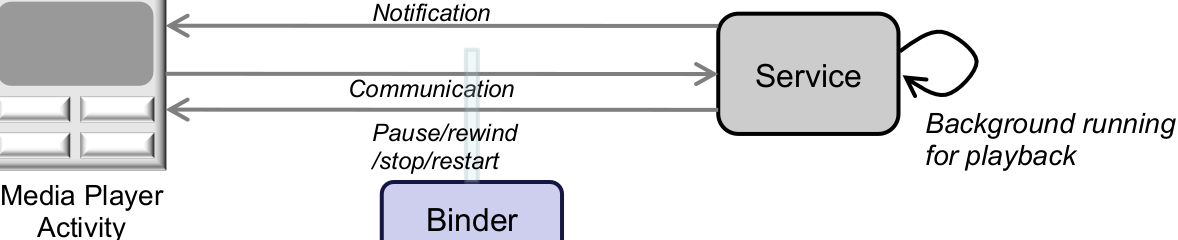
\includegraphics[width=0.15\textwidth]{android/service_example.png}

Service have their own lifecycle. Typically start one or more threads to
perform work outside the UI tread. Always stop services to avoid wasting
resources and consuming battery power. A started service handling requests
sequentially can be implemented by extending the IntentService class

\subsection{Broadcast Receiver}
Component that receives and reacts to broadcast announcements (<- are Intents too).
Many broadcasts originate in system code (E.g., announcements that the time
zone has changed, that the battery is low. Incoming SMS)
Receiver are implemented by extending BroadcastReceiver.

Register in AndroidManifest (in many cases are permissions needed):

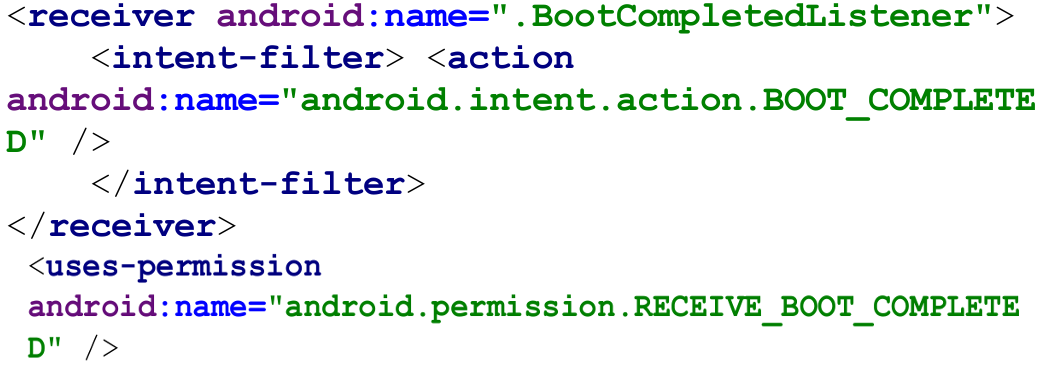
\includegraphics[width=0.15\textwidth]{android/broadcast_receiver.png}

\begin{lstlisting}
public class BootCompletedListener extends BroadcastReceiver {
 @Override
 public void onReceive(Context context, Intent intent) {
  // do something, when boot has completed
 }
}
\end{lstlisting}

\subsection{Content Provider}
recommended way to share data between Android applications (E.g. address book,
photo gallery). Represented by URI and MIME type.
Applications do not call content providers directly (may only to read). They
call ContentResolvers instead as they typically do not reside in the same
process.
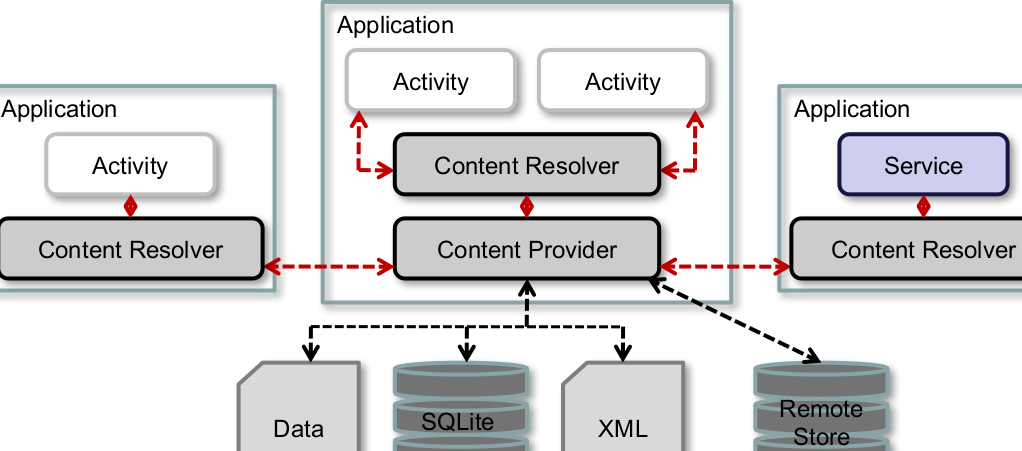
\includegraphics[width=0.15\textwidth]{android/content_provider.png}

\textbf{Android content provider} $ContactsContract$: All kinds of personal
data: phone numbers, email addresses etc.. $MediaStore$: Meta data for all
available media on both internal and external storage devices. $Browser$:
Bookmarks, search results, etc. $CallLog$: Information about placed and
received calls. $Settings$: Global system-level device preferences.

The ContentProvider can be accessed from several programs at the same time,
therefore you must implement the access \textbf{thread-safe}. E.g. add
$synchronized$ to the methods.

\textbf{Content URIs}: addresses for public content.
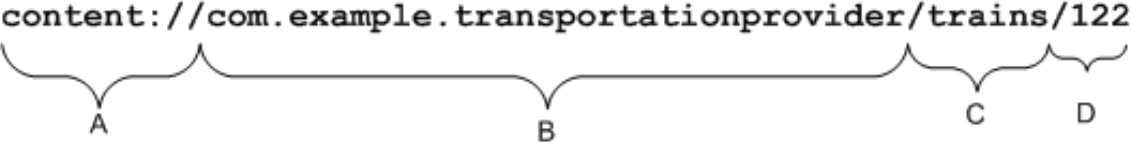
\includegraphics[width=0.15\textwidth]{android/content_uri.png}
A: prefix indicating that the data is controlled by a content provider. B:
authority part; identifies the content provider. C: path to determine what kind
of data is being requested. D: ID of the specific record being requested
(optional).

\textbf{Summary}: Queries to content providers return cursors. Modifying data
in a content provider by inserts, updates, and deletes goes through content
resolver. Implementing a content provider requires extending the
ContentProvider class, overwriting six methods and declaring the content
provider in the Android manifest.

\subsection{Processes and Threads}
\textbf{Default:} Applications run in a single Linux process. All components of
an application (activities, services, content providers, etc.) share this
process. These components also share a single thread of execution (“main
thread” or “UI thread”) within this process

\textbf{Processes may get killed} when memory is low. Which one to kill is
decided by an importance hierarchy.
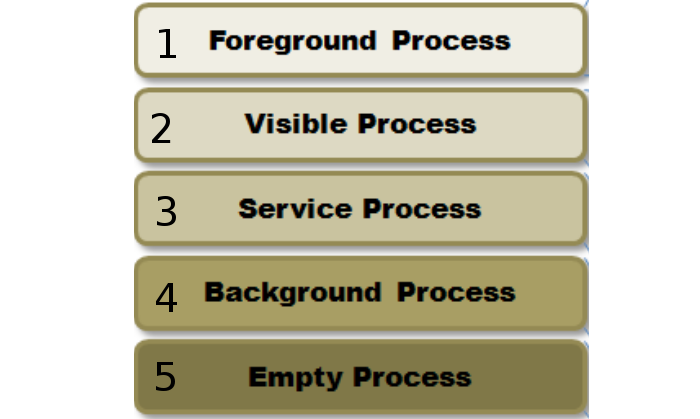
\includegraphics[width=0.15\textwidth]{android/importance_hierarchy_1.png}
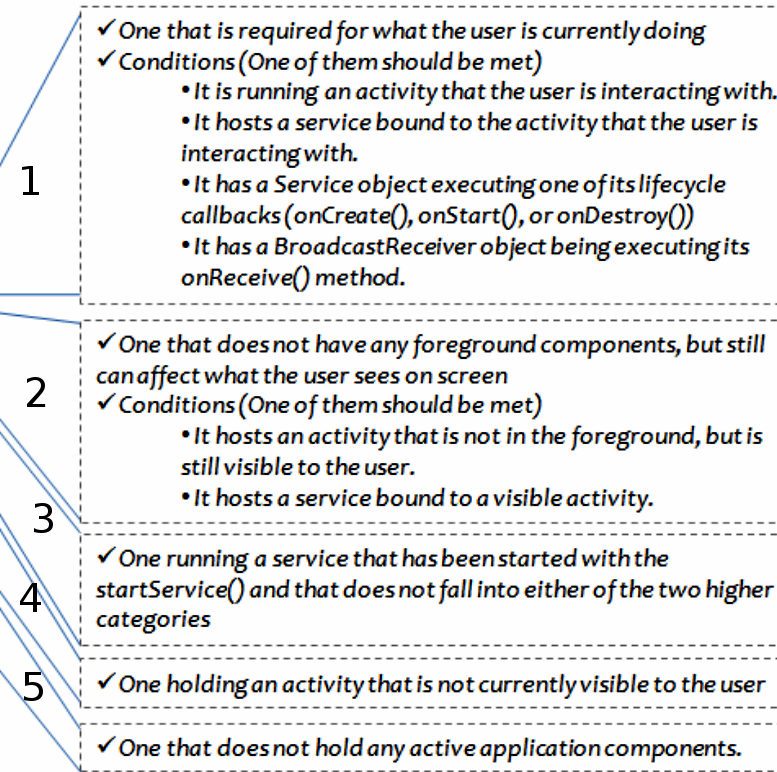
\includegraphics[width=0.15\textwidth]{android/importance_hierarchy_2.png}

Component ranking may increase if it contains components that serve components
in higher ranked processes. Thus, we recommend to create a service instead of
worker threads.

\textbf{UI Thread} is actually the \textbf{Main Thread}. It is called UI Thread
since all components are instantiated in it. Only this thread is supposed to
interact with the UI toolkit.

\textbf{Worker Thread} for long-lasting-operatins (To avoid infamous
“application not responding”). E.g. computations or downloads. To access
UI-Thread use: Activity.runOnUiThread(Runnable) or View.post(Runnable) or
View.postDelayed(Runnable, long).

\begin{lstlisting}
new Thread(new Runnable() {
public void run() {
 final Bitmap bitmap = load("http://...");
 mImageView.post(new Runnable() {
   public void run() {
    mImageView.setImageBitmap(bitmap);
   }
 });
}
}).start();
\end{lstlisting}

\textbf{Looper} can be used to transform normal thread in continuously running
thread. $prepare()$ transforms thread. $loop()$ starts loop. $quit()$ stops the
loop. The main ui thread is also created with the Looper
(Looper.getMainLooper() returns the looper). Instead of transforming a thread
the \textbf{HandlerThread} class can be used.\\

\textbf{AsyncTask}
Performs operation in background. Results from $doInBackground$ method are sent
to $onPostExecute$ method, which can update the UI Thread. Additionally
supports methods to report progress.

\textbf{Handler}
Can be used to register to a thread and provides a simple channel to send data
to this thread. Create a new instance of the Handler class in the $onCreate()$
method of your activity, the resulting Handler object can be used to transmit
data to the main thread by using: $sendMessage(Message)$ or
$sendEmptyMessage()$. Useful if you want to transmit data multiple times to the
main thread.

\subsection{Storing Data}
Multiple ways to store data are provided:
\subsubsection{Shared Preferences}
Provides a general framework that allows you to save and retrieve persistent
key-value pairs of primitive data types. The data will persist across user
sessions (even if your application is killed). Get Object with
$getPreferences()$ (if you need one file) or $getSharedPreferences()$ if you
need multiple files (distinguished by name).

\textbf{write} values by getting the editor with $edit()$ and call
$putString()$, $putBoolean()$, ... Don't forget to $commit()$ the values.

\textbf{read} with $getBoolean()$, $getString()$, ..

\subsubsection{Internal Storage}
By default, files saved to the internal storage are private to your
application. Other applications cannot access them (nor can the user). When the
user uninstalls your application, these files are removed.

\textbf{write}
\begin{lstlisting}
FileOutputStream fos = openFileOutput(FILENAME, Context.MODE\_PRIVATE);
fos.write(string.getBytes()); fos.close();
\end{lstlisting}

\textbf{read} call $openFileInput()$ with name of file, which returns a
$FileInputStream$. Then $read()$ and $close()$.

\textbf{Static files} Can be saved in res/raw and opened with
openRawResource(), passing the R.raw.<filename> resource ID.

\textbf{Cache files} Employ $getCacheDir()$ before opening. Recommended size <
1 MB. May get deleted when low on space.

\subsubsection{External Storage}
Reading from and writing to external storage (SD card or non-removable storage)
is supported by every Android- compatible device.

check storage availability with $getExternalStorageState$ and access your files
e.g. with $getExternalFilesDir()$.

\textbf{Shared files} getExternalStoragePublicDirectory() passing it the type
of public directory you want such as DIRECTORY\_MUSIC, DIRECTORY\_PICTURES.

\textbf{Cache files} getExternalCacheDir() to get the directory where cache
files can be stored.

\subsubsection{SQLite Databases}
The Android SDK includes a sqlite3 database tool that allows you to browse
table contents. Reads and writes go directly to a single ordinary file (Read /
Write Locks on the entire file).

Use a \textbf{database manager} to create, modify and query a private database.

\begin{lstlisting}
public class EventDBHelper extends SQLiteOpenHelper {
 private static final String DATABASE_NAME = "events.db";
 private static final int DATABASE_VERSION = 3;

 /** Create a helper object for the Events database */
 public EventDBHelper(Context ctx) {
  super(ctx, DATABASE_NAME, null, DATABASE_VERSION);
 }

 //create the database
 @Override
 public void onCreate(SQLiteDatabase db) {
  db.execSQL("CREATE TABLE " + TABLE_EVENTS + " ("
  + _ID + " INTEGER PRIMARY KEY AUTOINCREMENT, "
  + COL_TIME + " INTEGER,"
  + COL_NAME + " TEXT NOT NULL);");
 }

 // called if old version of databse is referenced
 @Override
 public void onUpgrade(SQLiteDatabase db, int oldVersion, int newVersion) {
  db.execSQL("DROP TABLE IF EXISTS " + TABLE_EVENTS);
  onCreate(db);
  // in production migrate the data to the new version!
 }
}
\end{lstlisting}

\textbf{modify data} with either raw queries or \textbf{structured query}
\begin{lstlisting}
// Insert a new record into the Events database
SQLiteDatabase db = eventDBHelper.getWritableDatabase();
// INSERT INTO TABLE_EVENTS (COL_TIME, COL_NAME)
VALUES (System.currentTimeMillis(), string);
ContentValues values = new ContentValues();
values.put(COL_TIME, System.currentTimeMillis());
values.put(COL_NAME, string);
db.insertOrThrow(TABLE_EVENTS, null, values);
\end{lstlisting}

\textbf{querying database (windowing)} prevents the system from having to load
all result data at a time and thus saves memory. Generally, cursors need to be
closed. A cursor can be registered at the Activity that performs the query. As
a consequence the Android system handles closing and re-querying when needed as
after lifecycle events such as onPause.

\begin{lstlisting}
SQLiteDatabase db = eventDBHelper.getReadableDatabase();
Cursor cursor = db.query(TABLE_EVENTS, FROM, null, null, null, null, ORDER_BY);
while (cursor.moveToNext()) {
 // Could use getColumnIndexOrThrow() to get indexes
 long id = cursor.getLong(0);
 long time = cursor.getLong(1);
}
\end{lstlisting}

\subsubsection{Network Connection}
To send and receive data you may employ the class HttpURLConnection.
Alternatively you may employ libraries such as Gson and OkHttp.

\begin{lstlisting}
URL url = new URL("http://www.android.com/");
HttpURLConnection urlConnection = (HttpURLConnection)
url.openConnection();
try {
  InputStream in = new BufferedInputStream(urlConnection.getInputStream());
  readStream(in);
  finally {
    urlConnection.disconnect();
  }
}
\end{lstlisting}

\subsection{Transferring Program Control / Intents}
\textbf{Intents:} (Passive object, Set of Strings). Used for transfering
control or notify components (VIEW, CALL, PLAY, ...). Systems matches Intent
with most suitable. It can be used to start an activity, start or communicate
with background service, send broadcast

\begin{lstlisting}
public void onClickSendBtn(final View btn){
  Intent intent = new Intent(this, Receiver.class);
  intent.putExtra("msg", "Hello World");
  startActivity(intent);
}
\end{lstlisting}

\textbf{Explicit Intent:} fully qualified class name of target. Mostly used for
internal messages of an application (starting an activity).

\textbf{Implicit Intent:} passive data structure holding an description of an
action to be performed. \textit{Action}: e.g. ACTION\_VIEW, ACTION\_EDIT.
\textit{Category:} category of component that should handle the intent (e.g.
browsable). \textit{Data:} URI and data type (MIME type). \textit{Extras}
Key-value pairs for additional information.

To \textbf{handle implicit intents} define intent filters in AndroidManifest.
Components without a filter can only receive explicit intents.

System \textbf{resolves implicit intent} by matching the most suitable
component (action, category, data). If multiple components match the filter,
the user can chose. If no component match, an exception is raised.

\textbf{resolution rules:}

\textit{Action}: if intent and filter has no action => fails. If filter has
action but intent not => match.

\textit{Category}: Every category of intent must match (but filter can contain
more)! DEFAULT is necessary to receive implicit intents. LAUNCHER category is
necessary if callable from launcher.

\textit{Data}: if 1) intent contains type and URI (or type can inferred from
URI) => filter matches if type and URI are the same.
2) Intent contains either type nor URI => filter matches if no type and URI are
defined
3) Intent contains URI but no type (and type can not be inferred) => filter
matches if URI matches and no type is defined.
4) Intent contains type but no URI => filter matches if type matches and no URI defined


\textbf{E.g. of Intent Filter in AndroidManifest}
\begin{lstlisting}
<activity android:name="SomeActivity">
  <intent-filter>
      <action android:name="android.intent.action.EDIT" />
      <category android:name="android.intent.category.DEFAULT" />
      <data android:scheme="http" android:type="video/*" />
  </intent-filter>
</activity>
\end{lstlisting}

Android uses a requestId to \textbf{return results from a sub-activity}:
\begin{lstlisting}
startActivityForResult(new Intent(this, A.class), i1);
startActivityForResult(new Intent(this, B.class), i2);

// in sub-activity A or B
setResult(resultCode, intent); finish();

// back in main activity
@Override
protected void onActivityResult(int requestCode, int resultCode, Intent
data) {
  switch (requestCode) {
    case i1: // result from call with i1
    if (resultCode == RESULT_OK) { /* ... */ }
    break;
    case i2: // result from call with i2
    if (resultCode == RESULT_OK) { /* ... */ }
    break;
  }
}
\end{lstlisting}

\textbf{Examples}
\begin{lstlisting}
Uri url = Uri.parse("http://www.domain.com");
// use file: or content: for other file types
Intent i = new Intent(android.content.Intent.ACTION_VIEW, url);
startActivity(i);
// if multiple browsers present, android will show choser (options: just once
or always)
\end{lstlisting}

\begin{lstlisting}
// GEO Location replace latitude & longitude
URI geoLocation = Uri.parse('geo:latitude,longitude')
Intent intent = new Intent(Intent.ACTION_VIEW);
intent.setData(geoLocation);
\end{lstlisting}

\begin{lstlisting}
// return number of possible activities
PackageManager pm = context.getPackageManager();
List<ResolveInfo> activities = pm.queryIntentActivities(intent, PackageManager.MATCH\_DEFAULT\_ONLY);
activities.size(); // <- possible activities
\end{lstlisting}

\subsection{Activity Lifecycle}
State of an activity is managed by the system.

System may:
1) move another activity into the foreground.
2) ask the activity to finish.
3) even simply kill its process.

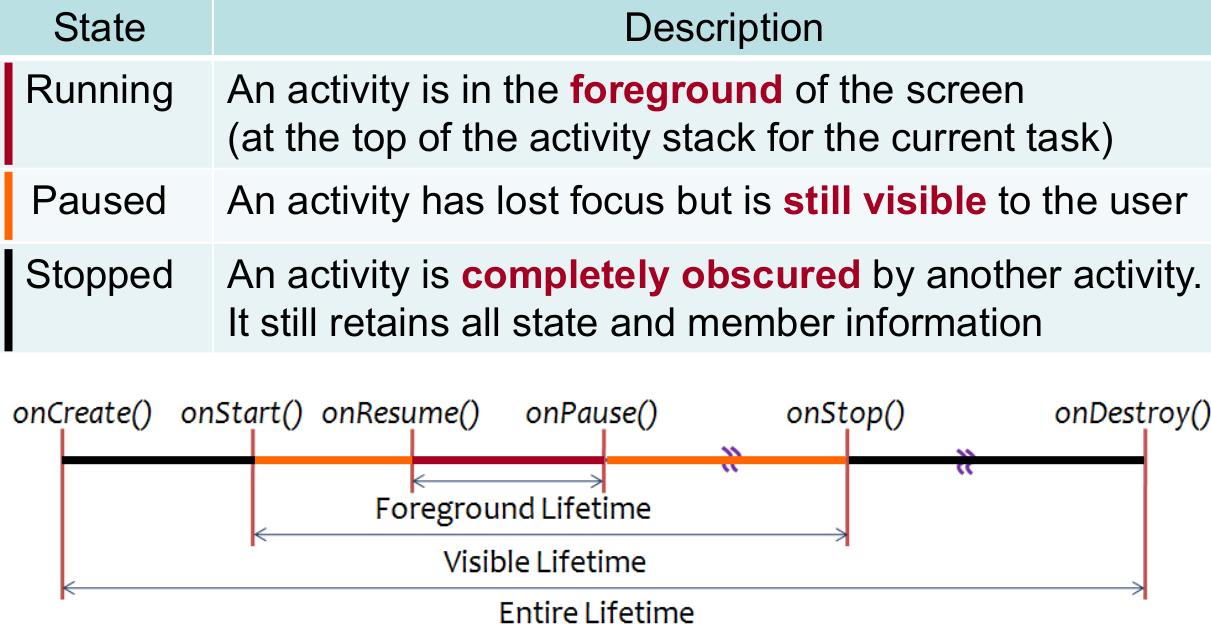
\includegraphics[width=0.15\textwidth]{android/activity_states.png}
System notifies an activity of a state transition by calling methods:
\textbf{onCreate:} first create or when activity was killed.
\textbf{onStart:} just before activity becomes visible.
\textbf{onRestart:} after activity has been stopped, to being started again.
\textbf{onResume:} before activity starts interacting with user (input goes to activity).
\textbf{onPause:} when about to resuming other activity (commit unsaved changes
here! stop animiations and CPU consumings)
\textbf{onStop:} when no longer visible to user (e.g. when destroyed or other activity resumed)
\textbf{onDestroy:} before destroy, but there is no guarantee.


\subsection{AndroidManifest}
Properties of Application: Name / ID (package), Version of App, Technical User
(sharedUserId), Required SDK, Required Privileges, Components
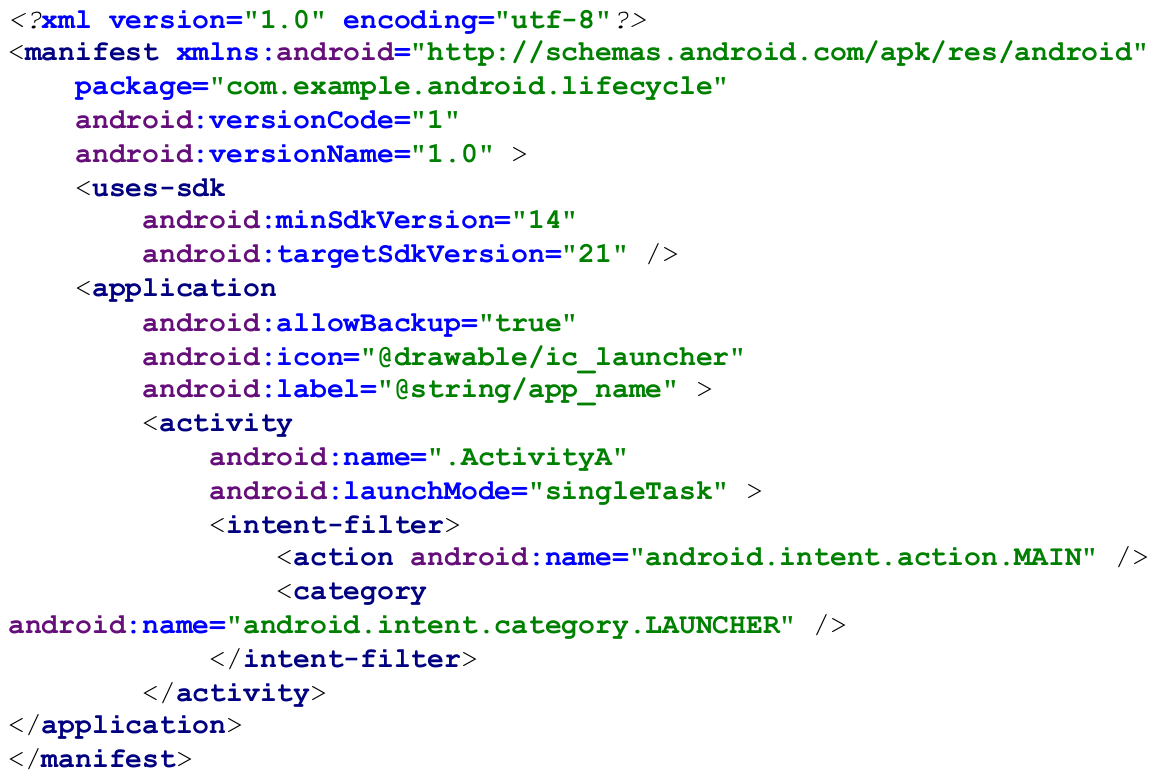
\includegraphics[width=0.15\textwidth]{android/manifest.png}
To be available from the launcher it must include an intent filter listening
for the MAIN action and the LAUNCHER category

\subsection{Configuration}
Advantages: Strings for localization, Images for different resolutions, Layouts for
different devices, ...

Seperated from code with resource files. Stored in \textbf{res} directory and
grouped by type: \textit{drawable}, \textit{layout}, \textit{values}. For
example \textit{res/values-de/strings.xml}
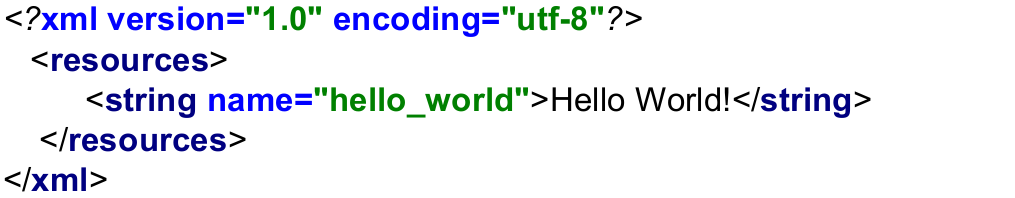
\includegraphics[width=0.15\textwidth]{android/example_resource.png}

Accessing resources in Java code with \textbf{wrapper class called R}, that
contains resource ids as static integers.

\begin{lstlisting}
// Load a custom layout for the current screen
setContentView(R.layout.main_screen);
// Set the text on a TextView object.
TextView view = (TextView)findViewByID(R.id.msg);
msgTextView.setText(R.string.hello_message);
// Set the title from a resource
this.getWindow().setTitle(Resources.getText(R.string.main_ title));
// Load a background for the current screen from a resource
this.getWindow().setBackgroundDrawableResource(R.drawable.my_background_image);
\end{lstlisting}

\subsection{Layout}
Defines the elements and their positioning on the user interface. Elements can
be declared in Java or XML. Advantages XML: seperation of presentation code.

Layout composed of \textbf{View} and \textbf{ViewGroups} (LinearLayout,
RelativeLayout, TableLayout, Gridlayout). ViewGroup contains other Views. Views
for interaction with User are called \textbf{Widgets} (Buttons, Check Boxes,
...). Good practice is to declare Layouts and UI elements in XML and to
instantiate them by creating Views and ViewGroups at run time.

Each view must define height and width with \textit{wrap\_content} or
\textit{fill\_parent}.
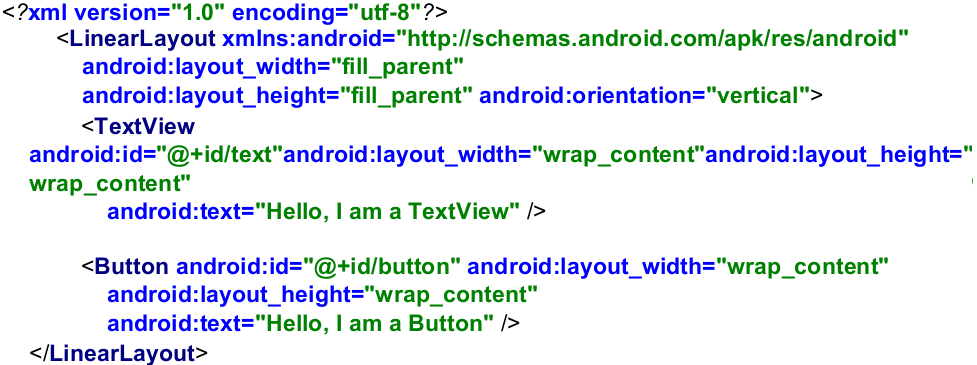
\includegraphics[width=0.15\textwidth]{android/view_example.png}

Handling UI Events like in Java Swing:
\begin{lstlisting}
// Capture our button from layout
Button button = (Button)findViewById(R.id.corky);
// Register the onClick listener with the impl. abovE
button.setOnClickListener(mCorkyListener);
\end{lstlisting}

\subsection{Development}
\textbf{Minimum Required SDK:} lowest version app supports.
\textbf{Target SDK:} Highest version app is tested for.
\textbf{Compile With:} Version against app is compiled.
\textbf{Theme:} Specific Android UI Theme.

\subsection{Testing}
\textbf{Local unit tests} run on developer’s machine. They should be written
with JUnit. They're located in $src/test/java$

\textbf{Instrumented tests} run on a device or emulator. They have access to
instrumentation information, such as the context of the app under test. They're
located in $src/androidTest/java$.

\subsubsection{Robolectric}
Robolectric is a unit test framework that simplifies writing Local Unit Tests
that depend on the Android SDK. Mocking code in the Android SDK is possible but
it means additional work.  Robolectric has done this for you. Tests run inside
the JVM on your workstation in seconds (as opposed to instrumented tests).
Robolectric handles inflation of views, resource loading and more. It runs
outside of emulator. And alternative is to use Mock Framework (e.g. Mockito).

\subsection{List}
ListActivity displays items by binding to a data source (\textbf{adapter}:
array, cursor). It consists of screen and row layout.
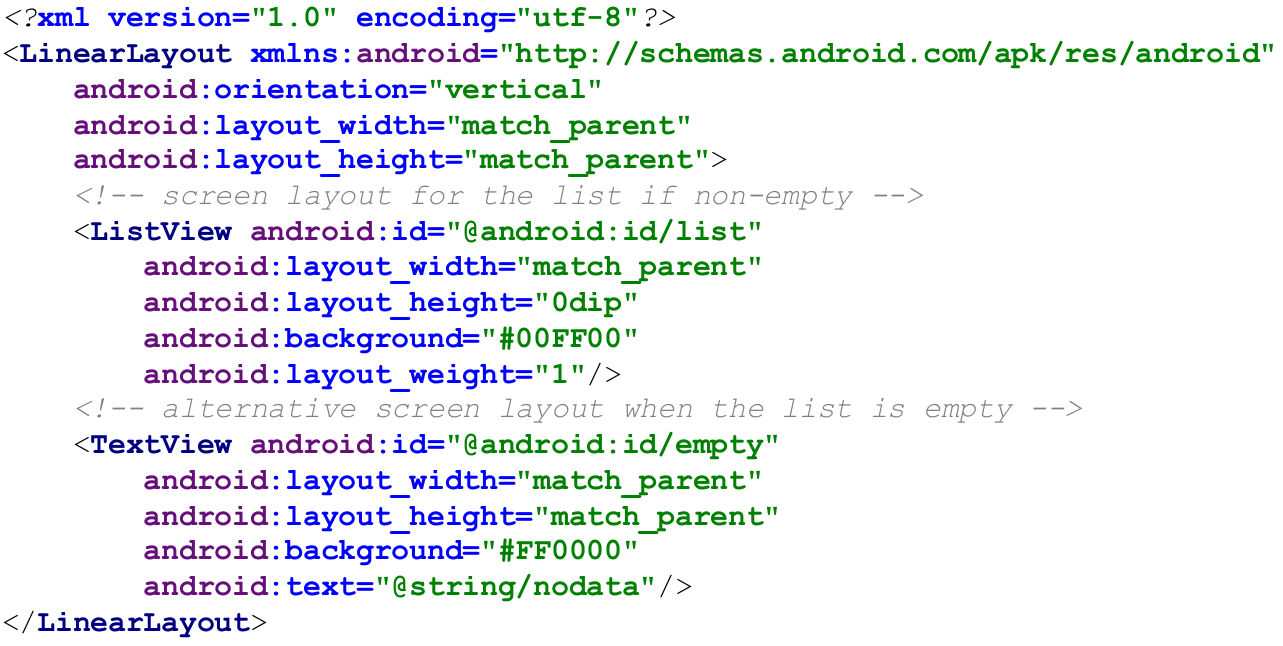
\includegraphics[width=0.15\textwidth]{android/list_layout_example.png}

Row Layout is defined when setting adapter. Define a own row layout or use
predefined built-in layouts (e.g. R.layout.simple\_list\_item\_1):
\begin{lstlisting}
setListAdapter(new ArrayAdapter<String>(this,
android.R.layout.simple_list_item_1, mValues););
\end{lstlisting}

onListItemClick:
\begin{lstlisting}
protected void onListItemClick(ListView l, View v, int position, long id)
\end{lstlisting}

To improve the \textbf{Performance} the \textbf{ViewHolder} pattern can be
used. It avoids frequent call of $findViewById$ during scrolling.
\begin{lstlisting}
static class ViewHolder { TextView text; }
@Override
public View getView(int position, View convertView, ViewGroup parent) {
  if(convertView==null){
    LayoutInflater inflater = ((Activity) mContext).getLayoutInflater();
      convertView = inflater.inflate(layoutResourceId, parent, false);
      viewHolder = new ViewHolderItem();
      viewHolder.text = (TextView) convertView.findViewById(R.id.textViewItem);
      convertView.setTag(viewHolder);
    } else { viewHolder = (ViewHolderItem) convertView.getTag(); }
    // modify value of viewHolder
}
\end{lstlisting}


\subsection{Recycler View}
more sophisticated alternative to display lists and grids (Fast scrolling
through large lists, Items are added or removed at run-time, Item add or
removal is to be animated)

Optimizations and enhancements come from:
1) a ViewHolder inner class in the adapter holding references to the views of
an individual item.
2) use of notification methods for item add or removal
3) possibilites to define animations by overwriting classes such as
RecyclerView.ItemAnimator

\subsection{Fragments}
Fragments are small chunks of the UI. They have their own layout and can be
inserted to an activity (by adding <fragment> element to the activity
declaration in XML, or from Java code by adding it to an existing ViewGroup).

\textbf{Advantages:} Can be reused in multiple activities. They have their own
\textit{backstack} and \textit{lifecycle} (usually implement at least:
onCreate, onCreateView and onPause).

\textbf{Example}
To show more details in landscape use create a xml layout for both orientations
(with same name). Landscape contains $android:orientation="horizontal"$ and a
FrameLayout for details:
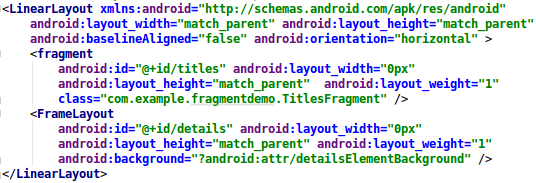
\includegraphics[width=0.15\textwidth]{android/fragment_details.png}

Check in ListFragment if details element is visible and use
\textbf{FragmentManager} to set it:
\begin{lstlisting}
public class TitlesFragment extends ListFragment {
  // check if details fragment visible
  View detailsFrame = getActivity().findViewById(R.id.details);
  landscape = detailsFrame != null && detailsFrame.getVisibility() == View.VISIBLE;
  // create details fragment if landscape is true
  details = DetailsFragment.newInstance(index);
  FragmentTransaction ft = getFragmentManager().beginTransaction();
  ft.replace(R.id.details, details);
  ft.setTransition(FragmentTransaction.TRANSIT_FRAGMENT_FADE);
  ft.commit();
\end{lstlisting}

\textbf{Useful subclasses of Fragments:}
\textit{DialogFragment} (Floating Dialog. Good alternativ to default Dialog,
since it works with back-stack).  \textit{ListFragment}.
\textit{PreferenceFragment} (Displays a hierarchy of Preference objects as a
list, Follows the visual style of system preferences).

\textbf{Communication:}
To be modular and decoupled any communication between fragments needs to go
through the hosting activity. To decouple communication fragment defines
interface which the activity implements:

\begin{lstlisting}
public class MyListFragment extends ListFragment {
  private OnItemSelectedListener listener;
  public interface OnItemSelectedListener {
    public void onRssItemSelected(String link);
  }
  public void onAttach(Activity activity) {
    super.onAttach(activity);
    listener = (OnItemSelectedListener) activity;
  }
  public void onListItemClick(ListView l, View v, int position, long id) {
    String title = l.getItemAtPosition(position).toString();
    RssItem rssItem = list.get(position);
    listener.onRssItemSelected(rssItem.getTitle());
    super.onListItemClick(l, v, position, id);
  }
\end{lstlisting}

\subsection{Application Menus}
Three types: Options menu, Context menu, Popup menu

\subsection{Android Action Bar}
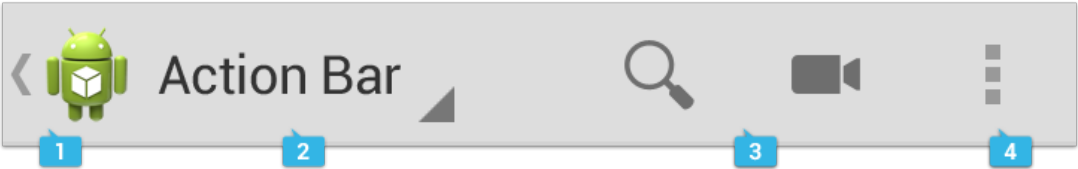
\includegraphics[width=0.15\textwidth]{android/actionbar.png}
1) app icon
2) view control
3) action button
4) overflow button

\textbf{Guidelines for Action Buttons}
Order by importance. Standard icons. Consider frequent, important and typical
actions. Buttons should not take more than 50\% of width. Not too many icons.

\textbf{Fragments} may contribute actions buttons with $hasOptionsMenu$ in
$onCreate$. Android calls $onCreateOptionsMenu$ in the fragment.

\subsection{MVC -  Model-View-Controller}
Model = represents app's data, notifies the controller about changes in the data, takes care of things like persistence, model objects and networking. View(UIView) = represents the face of the app, notifies the controller about user-actions, reusable classes without domain-specific logic. Controller(UIKit-dependent) = mediates between model and view, implements domain-specific logic, updates model and view. Problems = Tight coupling between View and ViewController, Controller is hard to test because of UIKit dependency, MVC == Massive View Controller = Delegate / DataSource methods, Target-Action methods, ViewController Lifecycle methods, Layout code, Formatting of data (transforming data object into strings), providing default values for missing data (placeholder images)
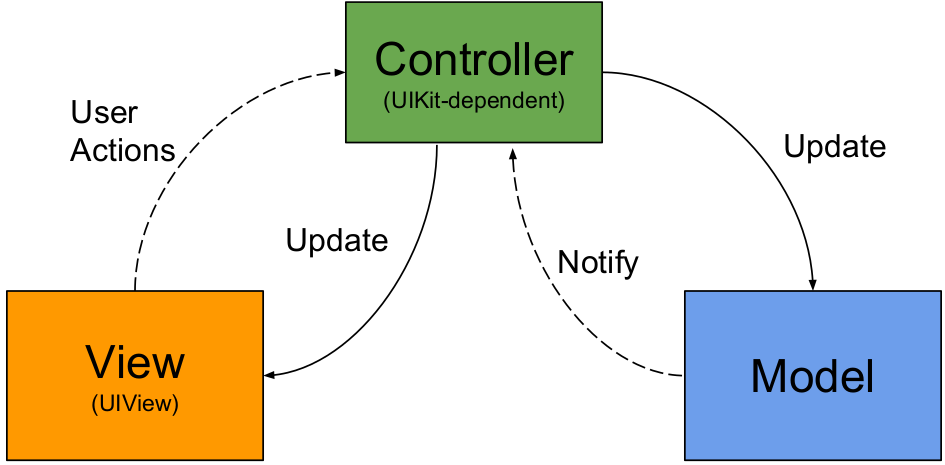
\includegraphics[width=0.15\textwidth]{mvc.png}
\textbf{Model}
Represents the app's data,
Notifies the controller about changes in the data,
Takes care of things like persistence, model objects and networking.

\textbf{View (UIView)}
Represents the face of the app,
Notifies the controller about user-actions,
Reusable classes without domain-specific logic.

\textbf{Controller (UIKit-dependent)}
Mediates between Model and View,
Implements domain-specific logic,
Updates Model and View

\textbf{Problems}
Tight Coupling between View and View Controller,
Controller is hard to test because of UIKit dependency,
MVC == Massive View Controller (Delegate / DataSource methods, Target-Action
methods, ViewController Lifecycle methods, Layout-Code, Formatting of data)

\subsection{MVP - Model-View-Presenter}
Model = represents app's data, notifies the controller about changes in the data, takes care of things like persistence, model objects and networking. View (UIView + UIViewController) = Represents the face of the app, Notifies the presenter about user-actions, \textbf{knows the presenter}. Presenter(UIKit-independent) = mediates between model and view, implements domain-specific logic, updates model and view, \textbf{Loosely coupled to View via protocol}.
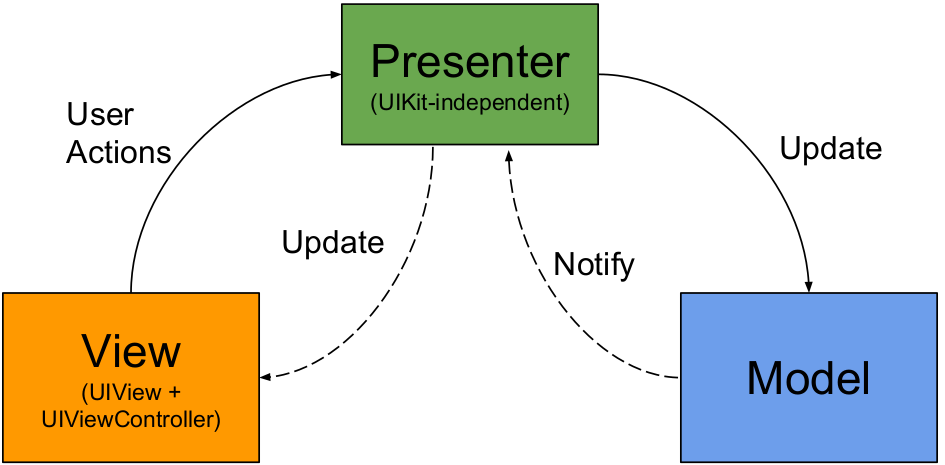
\includegraphics[width=0.15\textwidth]{mvp.png}
\textbf{Model} (same as in MVC)

\textbf{View (UIView + UIViewController)}
Represents the face of the app,
Notifies the presenter about user-actions,
Knows the presenter

\textbf{Presentor (UIKit-independent)}
Mediates between Model and View,
Implements domain-specific logic,
Updates Model and View,
Loosely coupled to View via protocol

\subsection{MVVM - Model-View-ViewModel}
Modle = represents the app's data, notifies the controller about changes in the data, takes care of things like persistence, model objects and networking. View (UIView + UIViewController) = represents the face of the app, \textbf{notifies ViewModel about user-actions and observes properties of ViewModel, Knows the ViewModel}. ViewModel(UIKit-independent) = mediates between Model and View, Implements domain-specific logic, updates model and view (indirectly via bindings), \textbf{loosely coupled to view via bindings / Observer-pattern}.
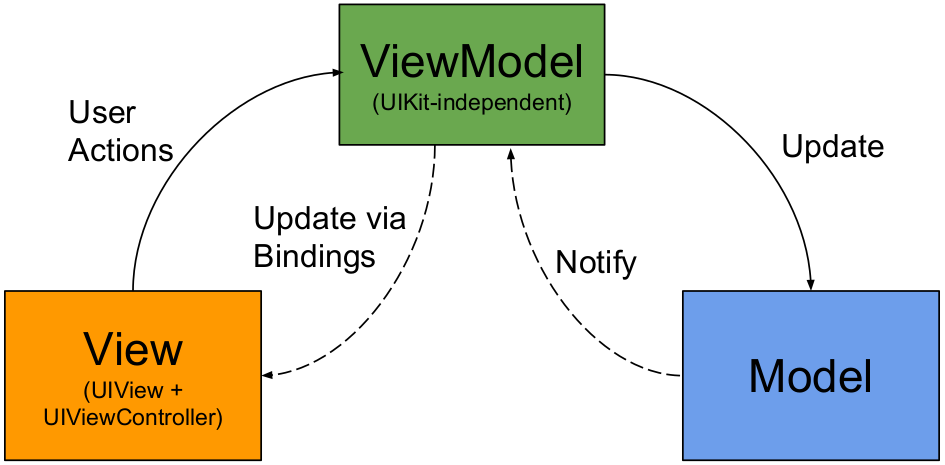
\includegraphics[width=0.15\textwidth]{mvvm.png}

\textbf{Model} (same as in MVC)

\textbf{View (UIView + UIViewController)}
face of the app,
Notifies ViewModel about user-actions and observes properties of ViewModel
Knows the ViewModel

\textbf{ViewModel (UIKit-independent)}
Mediates between Model and View,
Implements domain-specific logic,
Updates Model and View (indirectly via Bindings),
Loosely coupled to View via Bindings / Observer-Pattern


\subsection{Target-Action Pattern}
he target is an object that implements the action method
The action is a selector (basically a glorified string) that describes the name /
signature of that method
The button stores the target-action pairs
When the button is pressed, it looks for all the target-action pairs for the
touchUpInside Event and sends the corresponding action-selector to each target.
method dispatch happens dynamically requires Objective-C runtime
target object must be subclass of NSObject

\subsection{Richtig oder Falsch?}
\subsubsection{Komplett Richtig}
Android ist ein Software Stack fuer mobile Geräte, der u.a. ein Betriebsystem,
Middleware und wichtige Anwendungen bereit stellt

Anwendungen von Drittanbietern stellen ihre API zur Verfügung, indem sie die
Komponenten ihrer Anwendung beim System registrieren.

Für das Options Menu können alle Menueinträge im XML definiert und später im
Java geladen werden.

Android bietet Adapter an, die unterliegende Daten auf GUI Elemente, wie Views
mappen

Um Zugriff auf Daten in einem Content Provider zu erhalten, kann es sein, dass
eine Referenz auf den Context benötigt wird.

Android Applikationen sind aus lose gebundenen Komponenten
aufgebaut welche über Intents interagieren

Alle Komponenten einer Android Applikation müssen im Android
Manifest registriert werden

Die Architektur von Android besteht aus einem Hardware
Adaption Layer, Core Libraries, welche in C/C++ geschrieben
sind, der Dalvik Virtual Machine, den Java Libraries, dem
Application Framework und den Applikationen

Es wird empfohlen Layouts und User-Interface Elemente in XML
zu deklarieren und dann diese Layouts und Interface Elemente
zur Laufzeit zu benutzen

Mit XML definierte Menus können mittels eines Adapters an eine
View gebunden werden

Android unterstützt das Einfügen von dynamisch erzeugten Views
und ViewGroups

Eine Managed Query an einen Content Provider führt dazu dass
Android den Cursor managt

Die Speicherung von Daten mittels SharedPreferences
funktioniert nur mit primitiven Datentypen wie Boolean, Float, Int,
Long, String

Die gemeinsame Nutzung von Daten in verschiedenen
Applikationen erfolgt in Android über Content Provider

Anwendungskomponenten und zugehörige Intentfilter, sowie eine White-List mit
dem Permissions einer Applikation müssen im Android Manifest deklariert werden.

Views, die in einem XML Layout enthalten sind, können zur Identifikation bei
Aufrufen mit einer ID versehen werden.

Eine Adapter Objekt kann als Bridge zwischen einer View und den der View
unterliegenden Daten fungieren.

Die Android Debug Bridge adb kann benutzt werden um auf die SQLite Datenbanken
eines Androidgeräts zuzugreifen.

Edits auf eine Shared Preference, welche nicht comitted wurden, sind nicht
persistent über Sessions hinweg.

Ein impliziter Intent ist eine abstrakte Beschreibung einer Operation, die
ausgeführt werden soll.

Logs aus verschiedenen Anwendungen unda us Teilen des Systems werden in einer
Serie von Ringpuffern gesammelt und können mit dem logcat Tool gefiltert und
angesehen werden.

\subsubsection{Falsch}
Auf den meisten Android Phones läuft die neueste Version von Android (Stand: 1.
Juli 2012)

Die schnellste Möglichkeit auf Android Ressourcen wie Bilder und Strings lesend
zuzugeifen ist per Direct Access

In Android können Layouts nur in XML deklariert werden

Android Apps dürfen auf die Geo-Location des Phones zugreifen, ohne dass der
User zustimmen muss.

Die Namen von SQLite Datenbank-Dateien müssen auf einem Androidgerät äber a1le
Applikationen hinwes eindeutig sein.

In Shared Preferences können alle möglichen Datentypen gespeichert werden.

Implizite Intents werden typischerweise flir Applikations-interne Messages
eingesetzt, wie z.B. von einer Activity um eine Unteractivity zu starten.

Android Applikationen können auf einem Geräte gedebuggt werden, ohne vorher
signiert worden zu sein.

Auf Android Ressourc en kann mittels Direct Access immer am
schnellsten zugegriffen werden

Strings, Dimension Values, Colors, Styles, und Layouts können in
Android nur in Ressourcen abgelegt werden

Android stellt für Datenbankmanipulationen explizite Commit und
Rollback Kommandos zur Verfügung

Content Provider werden über eine Internetadresse
angesprochen

Explizite Intents beschreiben im Wesentlichen eine Aufgabe, die
ausgeführt werden soll. Solche Intents spezifieren Action,
Category, Data und Extras und überlassen es dem System, die
am besten geeignete Komponente zur Ausführung dieser
Aufgabe zu finden

Der Android Software Stack besteht auf Hardware Adapation Layer, Core libraries
welche in Java geschrieben sind, eine JVM, ein Application Framework und
Anwendungen.

Explizite Intents ermöglichen eine lose Kopplung von Anwendungen.

Android Anwendungen können die GPS Location immer ohne Zustimmung des Benutzers
brauchen, wenn diese auf dem Gerät zur Verfügung gestellt werden kann

Alle Intent Filter müssen in XML deklariert werden.

\subsection{Typische Fragen}
(XML Layout und ein paar Attribute fehlen) Welche Attribute müssen an der
Stelle (1) minimal zu dieser Konfiguration hinzugefügt wer- den, damit das
Layout wie abgebildet auf einem Android-Phone dargestellt werden kann?

\begin{lstlisting}
android:layout\_width="fill\_parent"
android:layout\_height="wrap\_content"
android:orientation="vertical"
\end{lstlisting}

Aus welchem Grund wird dieser Text mittels einer Ressource konfigurierbar
gehalten?
\begin{lstlisting}
Having the string configurable we can support multiple languages
\end{lstlisting}

Welche Anweisung kann in Java verwendet werden, um eine Instanz des Buttons zu
erzeugen, welche auf der in XML deklarierten Layout Konfiguration basiert.
\begin{lstlisting}
Button surveyPauseButton = (Button) findViewById(R.id.bu_survey_pause);
\end{lstlisting}
